%!TEX root = ../crowd_hierarchies_v.1.3.tex

\section{Preliminaries}
\label{sec:prelims}
In this section we first describe our structured data domain, then describe entities and entity extraction queries or interfaces, along with the response and cost model for these queries. Then we focus on crowdsourced entity extraction using these interfaces and consider the problem of maximizing the number of extracted entities. In particular, we define the problem of {\em crowd entity extraction} over {\em structured domains} under budget constraints. Then, we formally introduce the challenge of dependencies across queries when extracting entities from structured domains, and finally, we present an overview of our proposed algorithmic framework.


\subsection{Structured Data Domain}
\label{sec:data-domain}

Let $\domain$ be a data domain described by a set of discrete attributes $\attributes = \{A_1, A_2, \dots, A_d\}$. Let $dom(A_i)$ denote the domain of each attribute $A_i  \in \attributes$. We focus on domains where each attribute $A_i$ is hierarchically organized. For example, consider the Eventbrite domain introduced in \Cref{sec:challenges}. The data domain $\domain$ corresponds to all events and the attributes describing the entities in $\domain$ are $\attributes = \{$``Event Type", ``Location", ``Date"$\}$. \Cref{fig:eventsdomain} shows the hierarchical organization of each attribute.

\begin{figure}[h]
	\begin{center}
	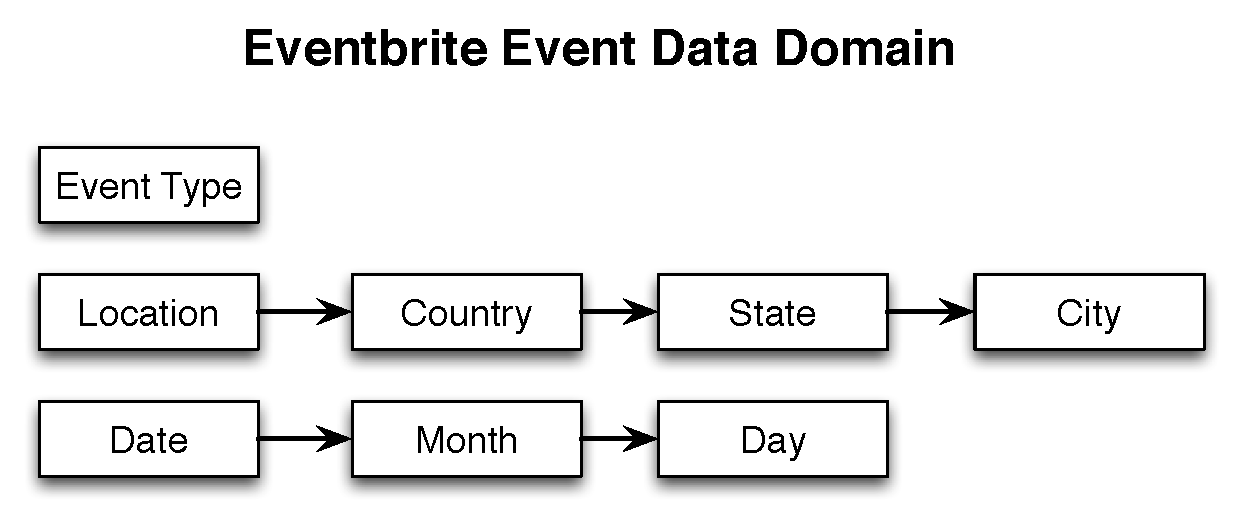
\includegraphics[clip,scale=0.33]{figs/eventsDomain.eps}
	\vspace{-10pt}
	\caption{The attributes describing the Eventbrite domain and the hierarchical structure of each attribute.}
	\label{fig:eventsdomain}
	\end{center}
	\vspace{-20pt}
\end{figure}

The domain $\domain$ can be viewed as a {\em poset}, i.e., a partially ordered set, corresponding to the cross-product of all available hierarchies\footnote{Note that $\domain$ is not a lattice since there is no unique infimum.}. Part of the poset corresponding to the previous example is shown in \Cref{fig:eventslattice}. We denote this cross-product as $\hierarchy$. As can be seen in \Cref{fig:eventslattice}, there are nodes, such as $\{\}$, where no attributes are specified, and nodes, such as $\{X1\}$ and $\{C1\}$ where just one of the attribute values is specified, as well as nodes, such as $\{X2, ST2\}$, where multiple attribute values are specified.

\begin{figure}[h]
\vspace{-10pt}
	\begin{center}
	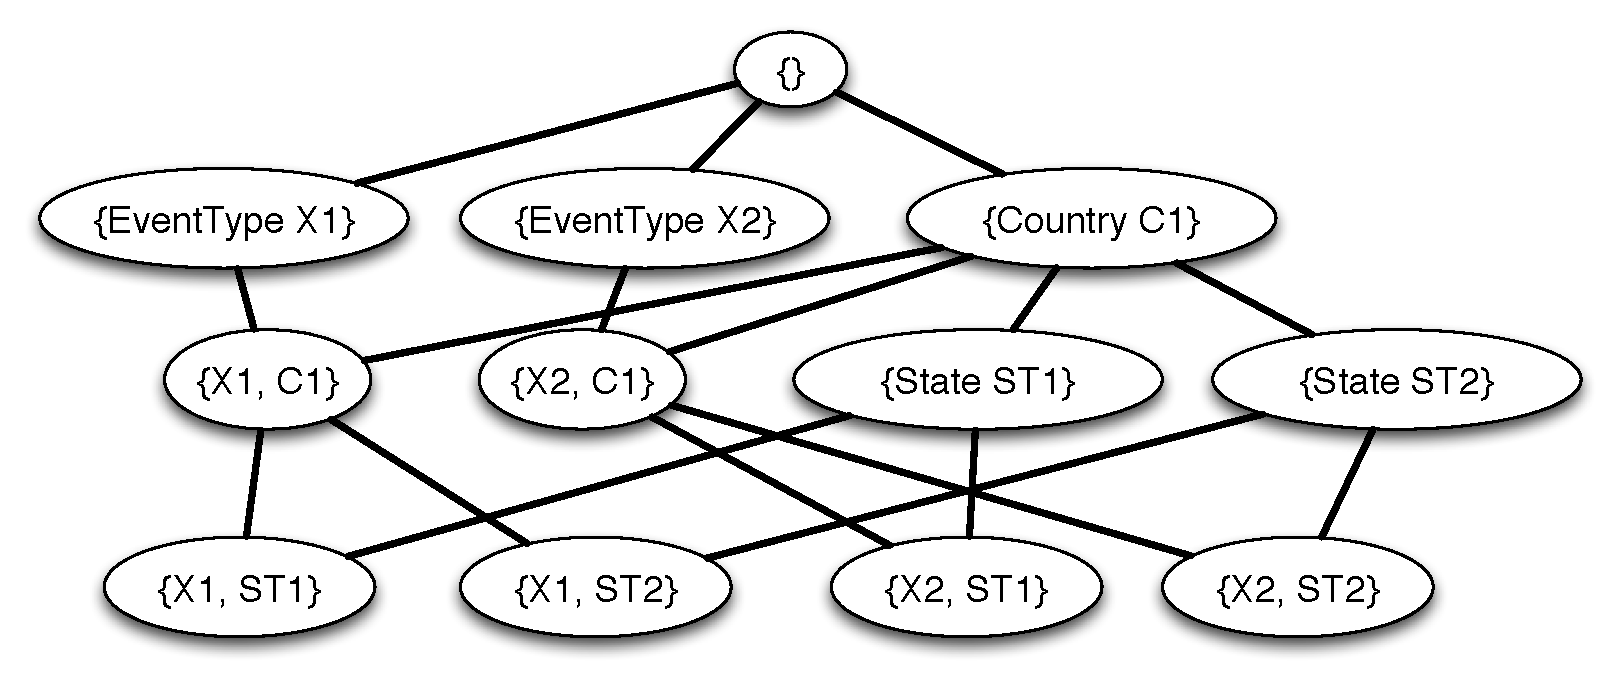
\includegraphics[clip,scale=0.32]{figs/eventsExLattice.eps}
	\vspace{-10pt}
	\caption{Part of the poset defining the entire event entity domain described by the attributes in \Cref{fig:eventsdomain}.}
	\label{fig:eventslattice}
	\end{center}
	\vspace{-20pt}
\end{figure}


\subsection{Entities and Entity Extraction Queries}
\label{sec:queries}

\stitle{Entities.} Our goal is to extract entities that belong to the domain $\domain$. We assume that each entity $e$ can be uniquely associated with one of the leaf nodes in the hierarchy $\hierarchy$; that is, there is a unique set of ``most-specific'' values of $A_1, \ldots, A_d$ for every entity. For example, in our Eventbrite dataset, each entity (here, a local event) takes place in a specific city, and on a specific day. Our techniques also work for the case when entities can be associated only with ``higher level'' nodes, but we focus on the former case for simplicity. 

\stitle{Queries.} Next, we describe queries for extracting entities from the crowd. First, a query $q$ is issued at a node $v \in \hierarchy$; that is, a query specifies zero or more attribute values from $A_1, \ldots, A_d$ that are derived from the corresponding values of $v$, implicitly requiring the worker to find entities that match the specified attribute values.  

Given a query issued at a node, there are three different configurations one can use to extract entities from the crowd: The first configuration corresponds to {\em single entity queries} where workers are required to provide ``one more" entity that match the specified attribute values mentioned in the query. Considering the Eventbrite example introduced in the previous section, an example of a single entity query would be asking a worker to provide ``a concert in Manhattan, New York". The second configuration corresponds to {\em queries of size k} where workers are asked to provide up to $k$ distinct entities. Finally, the last configuration corresponds to {\em exclude list queries}. Here,  workers are additionally provided with $l$ entities that have already been extracted and are required to provide up to $k$ distinct entities under the constraint that none of them is included in this exclude list of size $l$. It is easy to see that the last configuration generalizes the previous two. Therefore, in the remainder of the paper, we will only consider queries using the third configuration. To describe a query, we will use the notation $q(k,l)$ denoting a query of size $k$ accompanied with an exclude list of length $l$. 

\stitle{Query Response.} Given a query $q(k, l)$ issued at a node $v \in \hierarchy$, with an exclude list of entities $S, |S| = l$, a human worker gives us $k$ distinct entities that belong to the domain $\domain$, match the specified attribute values mentioned in the query (derived from $v$), and are not present in $S$. Furthermore, the human worker provides us the information for the attributes that are not specified in $q$ for each of the $k$ entities. For example, if our query is ``a concert in Manhattan, New York'', with $k = 1, l = 0$, the human worker gives us one concert in Manhattan, New York, but also gives us the day on which the concert will take place (here, the missing, unspecified attribute). If the query is ``a concert in the US'', with $k = 1, l = 0$, the human worker gives us one concert in the US, but also gives the day on which the concert will take place, as well as the specific city. If less than $k$ entities are present in the underlying population, workers have the flexibility to report either an empty answer or a smaller number of entities (\Cref{sec:neg}).

While the reader may wonder if getting additional attributes for entities is necessary, note that this information allows us to reason about which all nodes in $\hierarchy$ the entity belongs to; without this, it is impossible to effectively traverse the poset. Furthermore, we find that in most practical applications, it is useful to get the values of the missing attributes in order to organize and categorize the extracted entities better. Similar query interfaces that ask users to fully specify the attributes of entities they provide have been proposed in recent literature~\cite{quinn:2014}.

Workers may specify or extract an entity incorrectly. Such errors can be resolved by leveraging the presence of duplicate information and by applying de-duplication and entity resolution techniques. Resolving duplicate entities during extraction is crucial as this information is later used to estimate characterize the completeness of extracted entities, and thus, reason about the gain of additional queries.  At a high-level one can use an entity resolution or string similarity (e.g., jaccard coefficient) algorithm to identify duplicate entities. Furthermore, the additional attributes for each entity, can be used to further ascertain similarity of entities. We refer the user to Getoor and Machanavajjhala~\cite{getoor:kdd13} for an overview of entity resolution techniques. Finally, standard truth discovery techniques can be used to identify the correct attribute values for entities. Nevertheless entity resolution and truth discovery are orthogonal problems and not the focus of this paper. In our experiments on real datasets, we found that there were no cases where humans introduced errors to the attribute values of extracted entities. Only minor errors (e.g., misspelled entity names) were detected and fixed manually.

\stitle{Query Cost.} In a typical crowdsourcing marketplace, tasks have different costs depending on their difficulty. Thus, crowdsourced queries of different difficulties should also exhibit different costs. Let $c(\cdot)$ be a cost function for any query $q(k,l)$. This cost function should obey the following properties: (a) given a query with a fixed query size its cost should increase as the size of its exclude list is increasing, and (b) given a query with a fixed exclude list size its cost should increase as the number of requested answer increases. These are fixed upfront by the interface designer based on the amount of work involved.

\subsection{Crowdsourced Entity Extraction}
\label{sec:extraction}
The basic version of {\em crowdsourced entity extraction}~\cite{trushkowsky:2013} seeks to extract entities that belong to $\domain$, by simply using repeated queries at the root node, with $k = 1, l = 0$ (subsequent versions relax $l$ to be non-zero). However, when considering large entity domains, such as the event domain, one may need to issue a series of entity extraction queries at multiple nodes in  $\hierarchy$ --- often overlapping with each other --- so that the entire domain is covered. Issuing queries at different nodes ensures that the coverage across the domain will be maximized. 

We let $\pi$ denote a {\em querying policy}, that is, a chain of queries at different nodes in $\hierarchy$. Notice that multiple queries can be issued at the same node. Let $C(\pi)$ denote the overall cost, in terms of monetary cost (or equivalently, latency, since the more queries are issued, the more time the policy will take) of a querying policy $\pi$. We define the gain of a querying policy $\pi$ as the total number of unique entities, denoted by $\uentities(\pi)$ extracted when following policy $\pi$. Thus, there is a natural tradeoff between the gain (i.e., the number of extracted entities) and the cost of policies. 

Here, we require that the user will {\em only} provide a monetary budget $\tau_c$ imposing a constraint on the total cost of a selected querying policy, and optimize over all possible querying policies across different nodes of $\hierarchy$. Our goal is to identify the policy that maximizes the number of retrieved entities under the given budget constraint. More formally, we define the problem of budgeted crowd entity extraction as follows:

\begin{problem}[Budgeted Crowd Entity Extraction]
Let $\domain$ be a given entity domain and $\tau_c$ a monetary budget on the total cost of issued queries. The Budgeted Crowd Entity Extraction problem seeks to find a querying policy $\pi^*_S$ using queries over nodes in $\hierarchy$ that maximizes the number of unique entities extracted $\uentities(\pi^*_S)$ under the constraint $C(\pi^*_S) \leq \tau_c$.
\end{problem}
Notice that due to the different query configurations, the optimal querying policy for budgeted crowd entity extraction should also identify the optimal configuration $(k,l)$ for each query in $\pi^*_S$.

The cost of a querying policy $\pi$ is defined as the total cost of all queries issued by following $\pi$. We have that $C(\pi) = \sum_{q \in \pi} c(q)$ where the cost of each query $q$ is defined according to a cost model specified by the user. Computing the total cost of a policy $\pi$ is easy. However, the gain $\uentities(\pi)$ of a policy $\pi$ is unknown as we do not know in advance the entities corresponding to each node in $\hierarchy$, and hence, needs to be estimated, as we discuss next. 

It is easy to see that the problem of budgeted crowd entity extraction is an instance of a variant of the {\em stochastic knapsack problem}~\cite{kosuch,steinberg} where each item has a deterministic cost (weight) but a stochastic profit. The stochastic knapsack problem is known to be NP-hard, hence is the budgeted crowd entity extraction problem.
\subsection{Underlying Query Response Model}
\label{sec:sampling}
In order to reason about the occurrence of entities as response to specific queries, we need an underlying query response model. Our query response model is based on the notion of popularity.

\stitle{Popularities.} We assume that each underlying entity has a {\em fixed, unknown popularity value} with respect to crowd workers. Given a query $q(1, 0)$, asking for one entity and using an exclude list of size $0$, the probability that we will get entity $e$ that satisfies the constraints specified by $q$ is nothing but the popularity value of $e$ divided by the popularity value of all entities $e'$ that also satisfy the constraints in $q$. As an example, if there are only two entities $e_1, e_2$ that satisfy the constraints specified by a given query $q_1$, with popularity values $3$ and $2$,
then the probability that we get $e_1$ on issuing a query $q_1(1, 0)$ is 3/5. 
If an exclude list $S$ is specified, then the probability that we will get an entity $e \notin S$ is the popularity value of $e$ divided by the popularity values of all entities $e' \notin S$ also satisfying the constraints specified by $q$. Note that, we do not assume that all workers follow the same popularity distribution. Rather the overall popularity distribution can be seen as an average of the popularity distributions across all workers.

Thus, since workers are asked to provide a limited number of entities as response to a query, each entity extraction query can be viewed as taking a random sample from an unknown population of entities. In the rest of the paper, we will refer to the distribution characterizing the popularities of entities in a population of entities as the {\em popularity distribution} of the population. We note that this is equivalent to the underlying assumption in the species estimation literature~\cite{chao:1992} (\Cref{sec:gainestimators}).

% We assume that the underlying entities exhibit different {\em popularity levels} with respect to crowd workers. These popularity levels can be formally defined using the notion of a probability distribution. In particular, the probability that an entity will appear as part of a query result depends on its {\em popularity} relative to the overall entity population. The popularity of an entity for a query $q$ is defined as the probability that this entity will appear in a query $q(1,0)$, i.e., a query asking for one entity from the population and using an exclude list of size zero. Since workers are asked to provide a limited number of entities as response to a query, each entity extraction query can be viewed as taking a random sample from an unknown population of entities. In the remainder of the paper, we will refer to the distribution characterizing the popularities of entities corresponding to a population as the {\em popularity distribution} of the population. 

Then, estimating the gain of a query $q(k,l)$ at a node $v \in \hierarchy$ is equivalent to estimating the number of new entities extracted by taking additional samples from the population of $v$ given all the retrieved entities by past samples associated with node $v$~\cite{trushkowsky:2013}. 

\stitle{Samples for a Node.} When extracting entities,  the retrieved entities for a node $v$ can correspond to two different kinds of samples: (i) those that were extracted by considering the {\bf entire population} corresponding to node $v$ (ii) and those that we obtained by sampling {\bf only a part of the population} corresponding to $v$. Samples for a node $v$ can be obtained either by querying node $v$ or by indirect information flowing to $v$ by queries at other nodes. We refer to the latter case as {\em dependencies across queries}. 
\begin{figure}[h]
	\begin{center}
	\vspace{-10pt}
	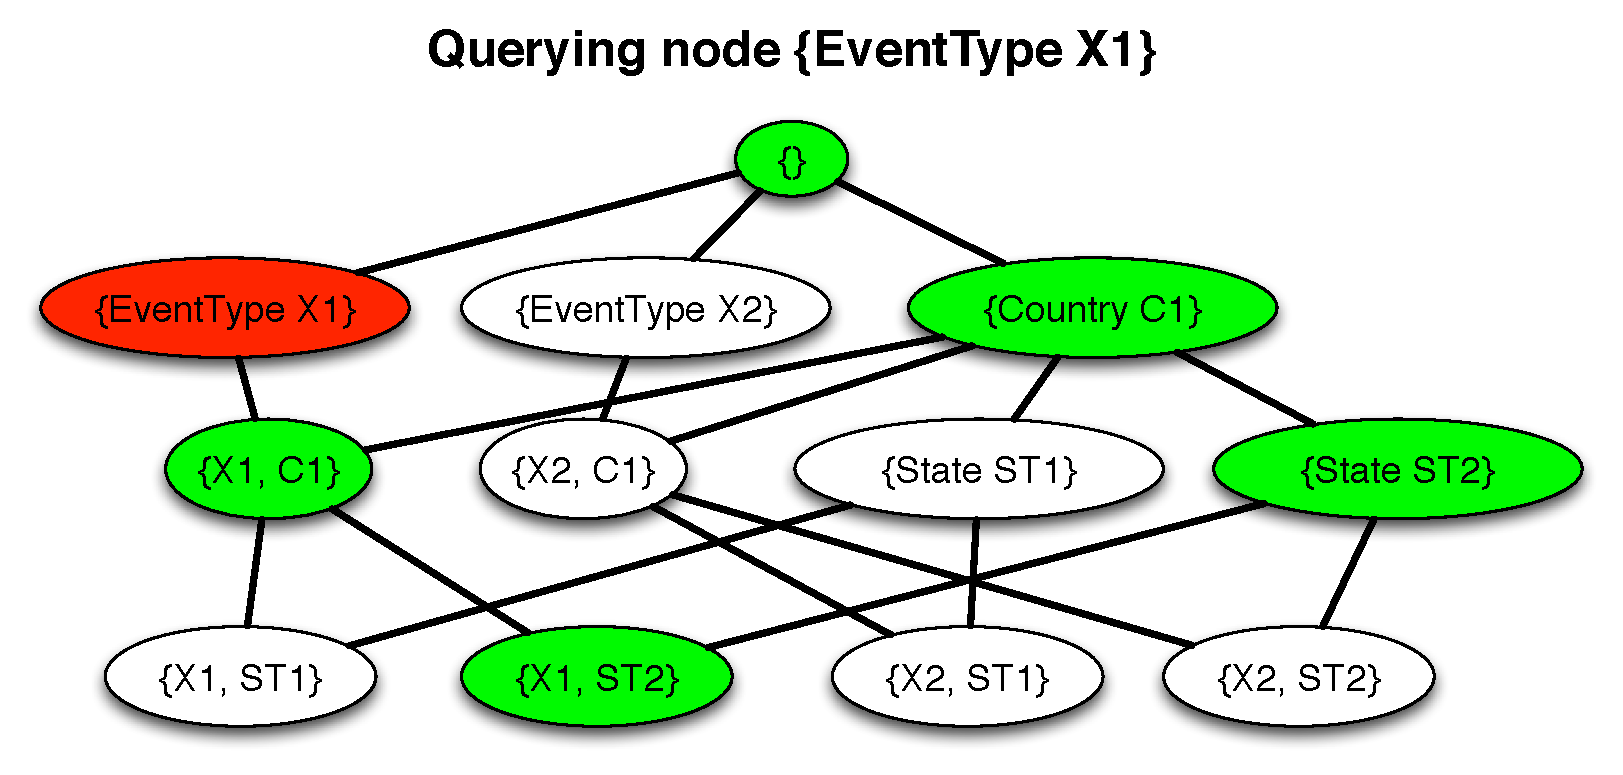
\includegraphics[clip,scale=0.3]{figs/exampleQuery.eps}
	\caption{An example query that extract an entity sample from the red node. The nodes marked with green correspond to the nodes for which indirect entity samples are retrieved.}
	\label{fig:query}
	\vspace{-10pt}
	\end{center}
	\vspace{-5pt}
\end{figure}

We use an example considering the poset in \Cref{fig:eventslattice}, to illustrate these two cases. The example is shown in \Cref{fig:query}. Assume a query $q(k,0)$ issued against node \{EventType X1\}. Assume that the query result contains entities that correspond only to node \{X1,ST2\}. The green nodes in \Cref{fig:query} are nodes for which samples are obtained indirectly without querying them. Notice, that all these nodes are ancestors of \{X1,ST2\}. Analyzing the samples for the different nodes we have:
\squishlist
\item The samples corresponding to nodes \{X1, C1\} and \{X1,ST2\} were obtained by considering their {\em entire population}. The reason is that node \{EventType X1\} is an ancestor of both and the entity population corresponding to it fully contains the populations of both \{X1,C1\} and \{X1,ST1\}. 
\item The samples corresponding to nodes \{ \}, \{Country C1\} and \{State ST2\} were obtained by considering only part of their population. The reason is that the population of node \{EventType X1\} does not fully contain the populations of these nodes. 
\squishend

Samples belonging to both types need to be considered when estimating the gain of a query at a node in $v \in \hierarchy$. To address this issue we merge the extracted entities for each node in $\hierarchy$ into a single sample and treat the unified sample as being extracted from the entire underlying population of the node. As we discuss later in \Cref{sec:solving} we develop querying strategies that traverse the poset $\hierarchy$ in a top-down approach, hence, the number of samples belonging in the first category, i.e., samples retrieved considering the entire population of a node, dominates the number of samples retrieved by considering only part of a node's population. Moreover, it has been shown by Hortal et al.~\cite{hortal2006evaluating} that several of the techniques that can be used to estimate the gain of a query (see \Cref{sec:gainestimators}) are insensitive to differences in the way the samples are aggregated.

\subsection{Framework Overview}
\label{sec:framework}
We present an overview of our proposed framework for solving the problem of budgeted crowd entity extraction over structured domains. We view the optimization problem described in \Cref{sec:extraction} as a multi-round adaptive optimization problem where at each round we solve the following subproblems: 
\squishlist 
\item \textbf{Estimating the Gain for a Query.} For each node in $v \in \hierarchy$, consider the retrieved entities associated with $v$ and estimate the number of new unique entities that will be retrieved if a new query $q(k,l)$ is issued at $v$. This needs to be repeated for all possible configurations of $k$ and $l$.
\item \textbf{Detecting the Optimal Querying Policy.} Using the gain estimates from the previous problem as input, identify the next (query, node) combination so that the total gain across all rounds is maximized with respect to the given budget constraint. 
\squishend
Our proposed framework iteratively solves the aforementioned problems until the entire budget is used. \Cref{fig:framework} shows a high-level diagram of our proposed framework.
% Throughout our framework, we assume that after issuing a query against the crowd, the retrieved answers can be associated with all relevant nodes across all attribute hierarchies, i.e., a worker will provide all the attribute values describing a reported entity. Dealing with incomplete information about entities is not the main focus of this paper and is part of the future work preposed in \Cref{sec:conclusions}.

\begin{figure}
	\begin{center}
	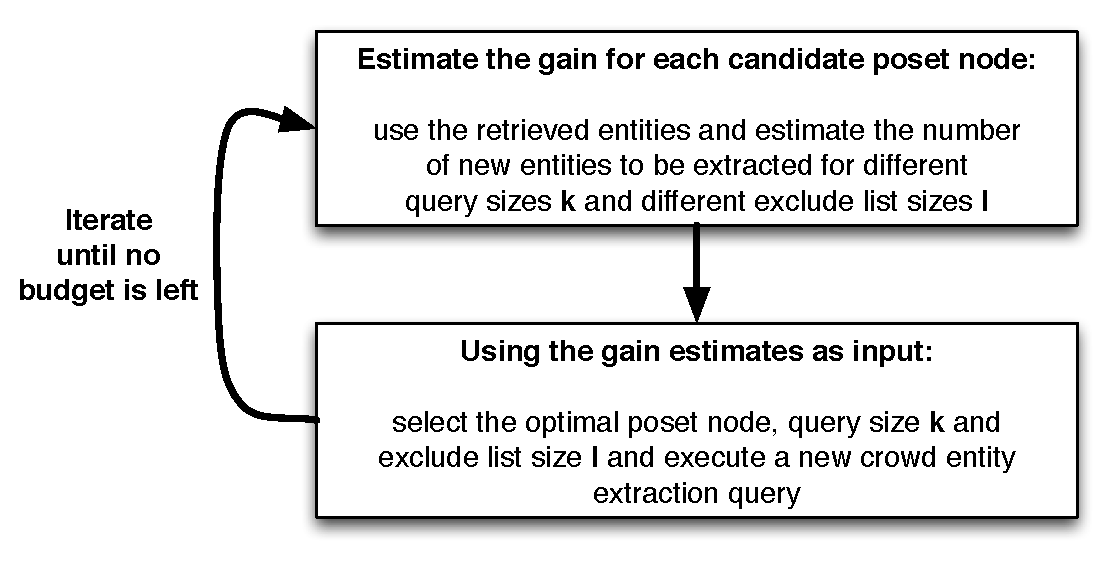
\includegraphics[clip,scale=0.43]{figs/framework.eps}
	\vspace{-10pt}
	\caption{Framework overview for budgeted entity extraction.}
	\label{fig:framework}
	\end{center}
	\vspace{-20pt}
\end{figure}
